\section{Auswertung}
\label{sec:Auswertung}

\subsection{Wheatston'sche Messbrücke}

\begin{table}
  \centering
  \caption{Messung von $R_3$ und $R_4$ für $R_{14}$}
  \label{tab:R14}
  \begin{tabular}{c c c c}
    \toprule
    $R_2$ & $R_3$ & $R_4$ & $R_14$ \\
    \midrule
     332 & 243 & 757 &  106,6 \\
     664 & 392 & 608 &  428,1 \\
    1000 & 612 & 388 & 1577,3 \\
    \bottomrule
  \end{tabular}
\end{table}

\begin{table}
  \centering
  \caption{Messung von $R_3$ und $R_4$ für $R_{13}$}
  \label{tab:R13}
  \begin{tabular}{c c c c}
    \toprule
    $R_2$ & $R_3$ & $R_4$ & $R_13$ \\
    \midrule
     332 & 579 & 421 &  456,6 \\
     664 & 595 & 405 &  975,5 \\
    1000 & 789 & 211 & 3739,3 \\
    \bottomrule
  \end{tabular}
\end{table}


\begin{figure}
  \centering
  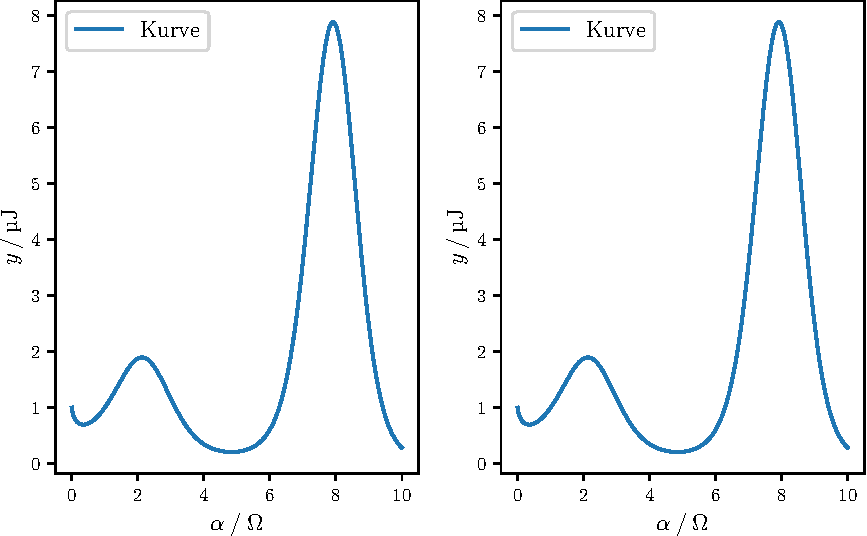
\includegraphics{plot.pdf}
  \caption{Plot.}
  \label{fig:plot}
\end{figure}


Siehe \autoref{fig:plot}!
